\section{Trimming trees}
\label{sct_trim}

Trimming a tree means cutting the nodes whose depth is larger than a specified threshold. Here is what will happen if I cut the catarrhini tree at depth 30:

\begin{center}
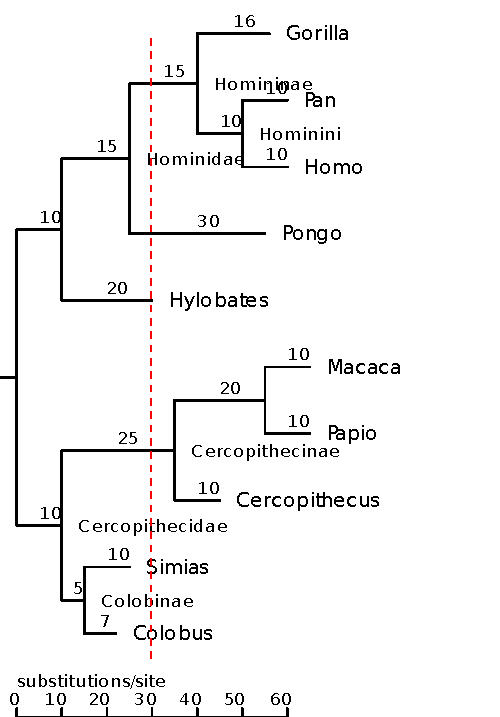
\includegraphics{trim_1.pdf}
\end{center}

\noindent{}The tree will be "cut" on the red line, and everything right of it will be discarded:

\verbatiminput{trim_2_svg.cmd}
\begin{center}
\includegraphics{trim_2_svg.pdf}
\end{center}

By default, depth is expressed in branch length units -- usually substitutions
per site. By passing the \texttt{-a} switch, it is measured in number of
ancestors, instead. Here are the first four levels of a huge tree (it has more than 1000 leaves):

\verbatiminput{trim_3_svg.cmd}
\begin{center}
\includegraphics{trim_3_svg.pdf}
\end{center}

\noindent{}The leaves with labels of the form \texttt{ID *} are also leaves in
the original tree, the other leaves are former inner nodes whose children got
trimmed.  Their labels are the (absolute) bootstrap support values of those
nodes. Note that the branch lengths are conserved. It is apparent that the
ingroup's lower half has very poor support. This would be harder to see wihout
trimming the tree, due to its huge size.

\subsubsection{Trimming cladograms}

By definition, cladograms do not have branch lengths, so you need to express depth in numbers of ancestors, and thus you want to pass \texttt{-a}.
